\begin{frame}
\frametitle{Processor evolution and software impact}

\begin{columns}[T] % align columns

\begin{column}{.48\textwidth}
\begin{figure}[htbp]
\begin{center}
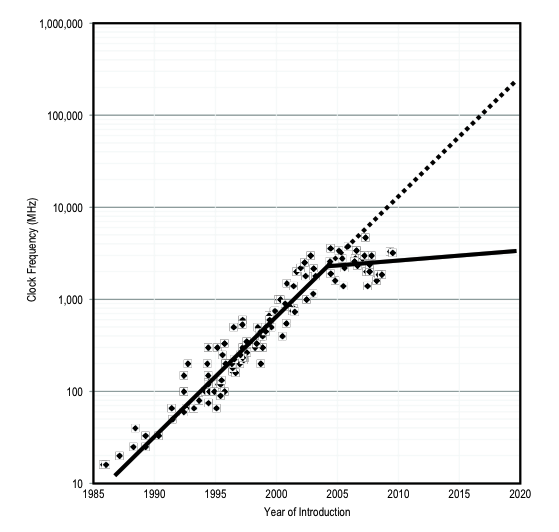
\includegraphics[width=1.0\textwidth]{images/moore2.png}
\end{center}
\end{figure}
\begin{center}
\small{Clock Frequency vs Time}
\end{center}
\end{column}%

\hfill%

\begin{column}{.48\textwidth}
\begin{itemize}
\item Single core performance has stalled, leading to multi/manycore and specialization
\item To even realize Moore's Law gains, we are pushed towards parallelization of algorithms and design for performance.
\item The software designs and implementations themselves need to evolve, not just be recompiled
\end{itemize}
\end{column}%

\end{columns}

\end{frame}


